\chapter*{Введение}
\addcontentsline{toc}{chapter}{Введение}

\textbf{Матрица} — это упорядоченный набор чисел, расположенных в виде таблицы. Этот математический объект находит широкое применение во многих областях науки, техники и естественных наук. Матрицы являются одним из основных инструментов в линейной алгебре и находят применение в решении различных математических задач.

\textbf{Умножение матриц} — есть операция вычисления матрицы, каждый элемент которой равен сумме произведений элементов в соответствующей строке первого множителя и столбце второго.

\textbf{Целью} данной лабораторной работы является анализ алгоритмов умножения матриц.

Необходимо выполнить следующие \textbf{задачи}:
\begin{enumerate}
    \item Изучить следующие алгоритмы умножения матриц: %поиска расстояния Левенштейна и Дамерау~---~Левенштейна.
    \begin{itemize}    
        \item классический алгоритм умножения;
        \item алгоритм Винограда;
        \item алгоритм Штрассена;        
        \item оптимизированный алогритм Винограда
    \end{itemize}
    \item Реализовать алгоритмы умножения матриц;%поиска редакционных расстояний.
    \item Выполнить замеры затрат реализаций алгоритмов по памяти;
    \item Выполнить замеры затрат реализаций алгоритмов по процессорному времени;
    \item Провести сравнительных анализ алгоритмов
\end{enumerate}

\chapter{Аналитическая часть}

\section{Классический алгоритм умножения}
Умножение матриц (обозначение: $AB$, реже со знаком умножения $A \times B$) — есть операция вычисления матрицы $C$, каждый элемент которой равен сумме произведений элементов в соответствующей строке первого множителя и столбце второго.

\begin{equation}
    \label{eq:classic_1}
    c_{ij} = \sum_{k=1}^{n}a_{ik}b_{kj} \quad (i = \overline{1, m}, j = \overline{1, p}),
\end{equation}

Классический алгоритм реализует формулу \ref{eq:classic_1}.

\section{Алгоритм Винограда}
Рассмотрим алгоритм Винограда, имеющий асимптотическую сложность $O(n^{2,3755})$~\cite{vinograd-haskell}.

Даны два вектора:
\begin{equation}
    U = (u_{1}, u_{2}, u_{3}, u_{4}),
\end{equation}
\begin{equation}
    V = (v_{1}, v_{2}, v_{3}, v_{4}).
\end{equation}
Их скалярное произведение равно:
\begin{equation}
    \label{eq:scalar_prod}
    U \times V = u_{1}v_{1} + u_{2}v_{2} + u_{3}v_{3} + u_{4}v_{4},
\end{equation}
что равносильно
\begin{equation}
    \label{eq:vinograd_1}
    U \times V = (u_{1} + v_{2})(u_{2} + v_{1}) + (u_{3} + v_{4})(u_{4} + v_{3}).
\end{equation}

Для упомянутых раннее матриц $A, B$ и $C$ скалярное произведение, по замыслу Винограда, \ref{eq:scalar_prod} можно свести к следующему выражению:
\begin{multline}
    \label{eq:vinograd_2}
    c_{ij} = \sum_{k = 1}^{n / 2}(a_{i,2k - 1} + b_{j, 2k})(a_{i,2k} + b_{j, 2k - 1}) - \\ - \sum_{k = 1}^{n / 2}a_{i,2k - 1}a_{i,2k} - \sum_{k = 1}^{n / 2}b_{2k - 1,j}b_{2k,j}.
\end{multline}
Для уменьшения количества арифметических операций Виноград предложил находить второе и третье слагаемое в \ref{eq:vinograd_2} заранее для каждой строки матрицы $A$ и каждого столбца матрицы \textit{B}.

Так, вычислив для \textit{i}-ой строки матрицы $A$ значение выражения

$\sum_{k = 1}^{n / 2}a_{i,2k - 1}a_{i,2k}$

можно использовать далее $n$ раз для нахождения элементов \textit{i}-ой строки матрицы $C$.  

Аналогично, вычислив для \textit{j}-ой столбца матрицы $B$ значение выражения

$\sum_{k = 1}^{n / 2}b_{2k - 1,j}b_{2k,j}$

можно использовать далее $n$ раз для нахождения элементов \textit{j}-ой столбца матрицы $C$.

Для примера, приведенного в формуле \ref{eq:vinograd_1}, в клаcсическом умножении производится четыре умножения и три сложения; в алоритме Винограда~--- шесть умножений и девять сложений. Но, несмотря на увеличение количества операций, выражение в правой части можно вычислить заранее и запомнить для каждой строки первой матрицы и каждого столбца второй матрицы.
Это позволит выполнить лишь два умножения и пять сложений, складывая затем только лишь с двумя предварительно вычисленными суммами соседних элементов текущих строк и столбцов. Операция сложения выполняется быстрее, поэтому на практике алгоритм должен работать быстрее классического алгоритма умножения матриц~\cite{vinograd-alg}.

При условии нечетного размера матрицы необходимо дополнительно добавить произведения крайних элементов соответствующих строк и столбцов.

\section{Алгоритм Штрассена}
Если добавить к матрицам $A$ и $B$ одинаковые нулевые строки и столбцы, их произведение станет равно матрице $AB$ с теми же добавленными строками и столбцами. Поэтому можно рассматривать только матрицы размера $n=2^k,\ k \in \mathbb{N}$, а другие случаи сводить к этому добавлением нулей, отчего $n$ может увеличиться лишь вдвое.

Пусть $A,B$ – матрицы размера $2^k \times 2^k$. Их можно представить как блочные матрицы размера $(2 \times 2)$ из $(2^{k-1} \times 2^{k-1})$–матриц:
\\~\\
$ 
A =
\begin{pmatrix}
A_{11} & A_{12} \\
A_{21} & A_{22}
\end{pmatrix}, \quad
B =
\begin{pmatrix}
B_{11} & B_{12} \\
B_{21} & B_{22}
\end{pmatrix}
$
\\~\\
По принципу блочного умножения, матрица $AB$ выражается через их произведение
\\~\\
$
AB
=
\begin{pmatrix}
A_{11} B_{11} + A_{12} B_{21} &
A_{11} B_{12} + A_{12} B_{22} \\
A_{21} B_{11} + A_{22} B_{21} &
A_{21} B_{12} + A_{22} B_{22}
\end{pmatrix}\ ,
$
\\~\\
где в правой части происходит восемь умножений матриц размера $2^{k-1} \times 2^{k-1}$. Поскольку матрицы образуют кольцо, то для вычисления правой части годится любой алгоритм умножения $(2 \times 2)$-матриц, использующий лишь сложения, вычитания и умножения. Штрассен предложил такой алгоритм с семью умножениями:


%\begin{align}
\begin{equation}
D = (A_{11} + A_{22}) (B_{11} + B_{22});
\end{equation}


\begin{equation}
D_1 = (A_{12} - A_{22}) (B_{21} + B_{22});
\end{equation}


\begin{equation}
D_2 = (A_{21} - A_{11}) (B_{11} + B_{12});
\end{equation}


\begin{equation}
H_1 = (A_{11} + A_{12}) B_{22};
\end{equation}


\begin{equation}
H_2 = (A_{21} + A_{22}) B_{11};
\end{equation}


\begin{equation}
V_1 = A_{22} (B_{21} - B_{11});
\end{equation}


\begin{equation}
V_2 = A_{11} (B_{12} - B_{22});
\end{equation}
\\~\\

\begin{multline}AB
=
\begin{pmatrix}
D & 0 \\
0 & D
\end{pmatrix}
+
\begin{pmatrix}
D_1 & 0 \\
0 & D_2
\end{pmatrix}
+
\begin{pmatrix}
-H_1 & H_1 \\
H_2 & -H_2
\end{pmatrix}
+
\begin{pmatrix}
V_1 & V_2 \\
V_1 & V_2
\end{pmatrix} \\
=
\begin{pmatrix}
D+D_1+V_1-H_1 & V_2+H_1 \\
V_1+H_2 & D+D_2+V_2-H_2
\end{pmatrix}\\
\end{multline}


Каждое умножение можно совершать рекурсивно по той же процедуре, а сложение – тривиально, складывая $(2^{k-1})^2$ элементов. Тогда время работы алгоритма $T(n)$ оценивается через рекуррентное соотношение:

$T(n) = 7 T(n/2) + O(n^2) = O(n^{\log_2 7})\ .$

\section{Оптимизированный алогритм Винограда}
В исследовательских целях, выполним следующие следующие оптимизации для алгоритма Винограда:
\begin{enumerate}
    \item сохранять значение $n / 2$, используемое в качестве ограничения цикла подсчета предварительных данных;
    \item операцию умножения на 2 заменить на побитовый сдвиг влево на 1;
    \item заменить операцию x = x + k на x += k
\end{enumerate}
\addcontentsline{toc}{section}{Вывод}
\section*{Вывод}
В данном разделе были рассмотрены следующие алгоритмы умножения матриц: %алгоритмы нахождения расстояния Левенштейна и Дамерау~---~Левенштейна.
\begin{itemize}    
    \item классический алгоритм умножения;
    \item алгоритм Винограда;
    \item алгоритм Штрассена;        
    \item оптимизированный алогритм Винограда
\end{itemize}
\clearpage

\chapter{Конструкторская часть}
В данном разделе будут приведены схемы алгоритмов умножения матриц, описание используемых типов данных и структуры программного обеспечения.

\section{Требования к программному обеспечению}

К программе предъявлен ряд функциональных требований:

\begin{itemize}
    \item наличие интерфейса для выбора действий;
    \item возможность ввода чисел, используя текстовые файлы;
    \item возможность произвести замеры процессорного времени работы;реализованных алгоритмов умножения матриц
\end{itemize}

\section{Разработка алгоритмов}


На рисунке \ref{fig:classic} представлена схема алгоритма классического умножения.

На рисунках \ref{fig:vinograd}--\ref{fig:vinograd} приведена схема алгоритма Винограда.

На рисунках \ref{fig:vinograd_opt}--\ref{fig:vinograd_opt2} представлена схема оптимизированного алгоритма Винограда.

На рисунке \ref{fig:strass} представлена схема алгоритма Штрассена.

\begin{figure}[h]
	\centering
	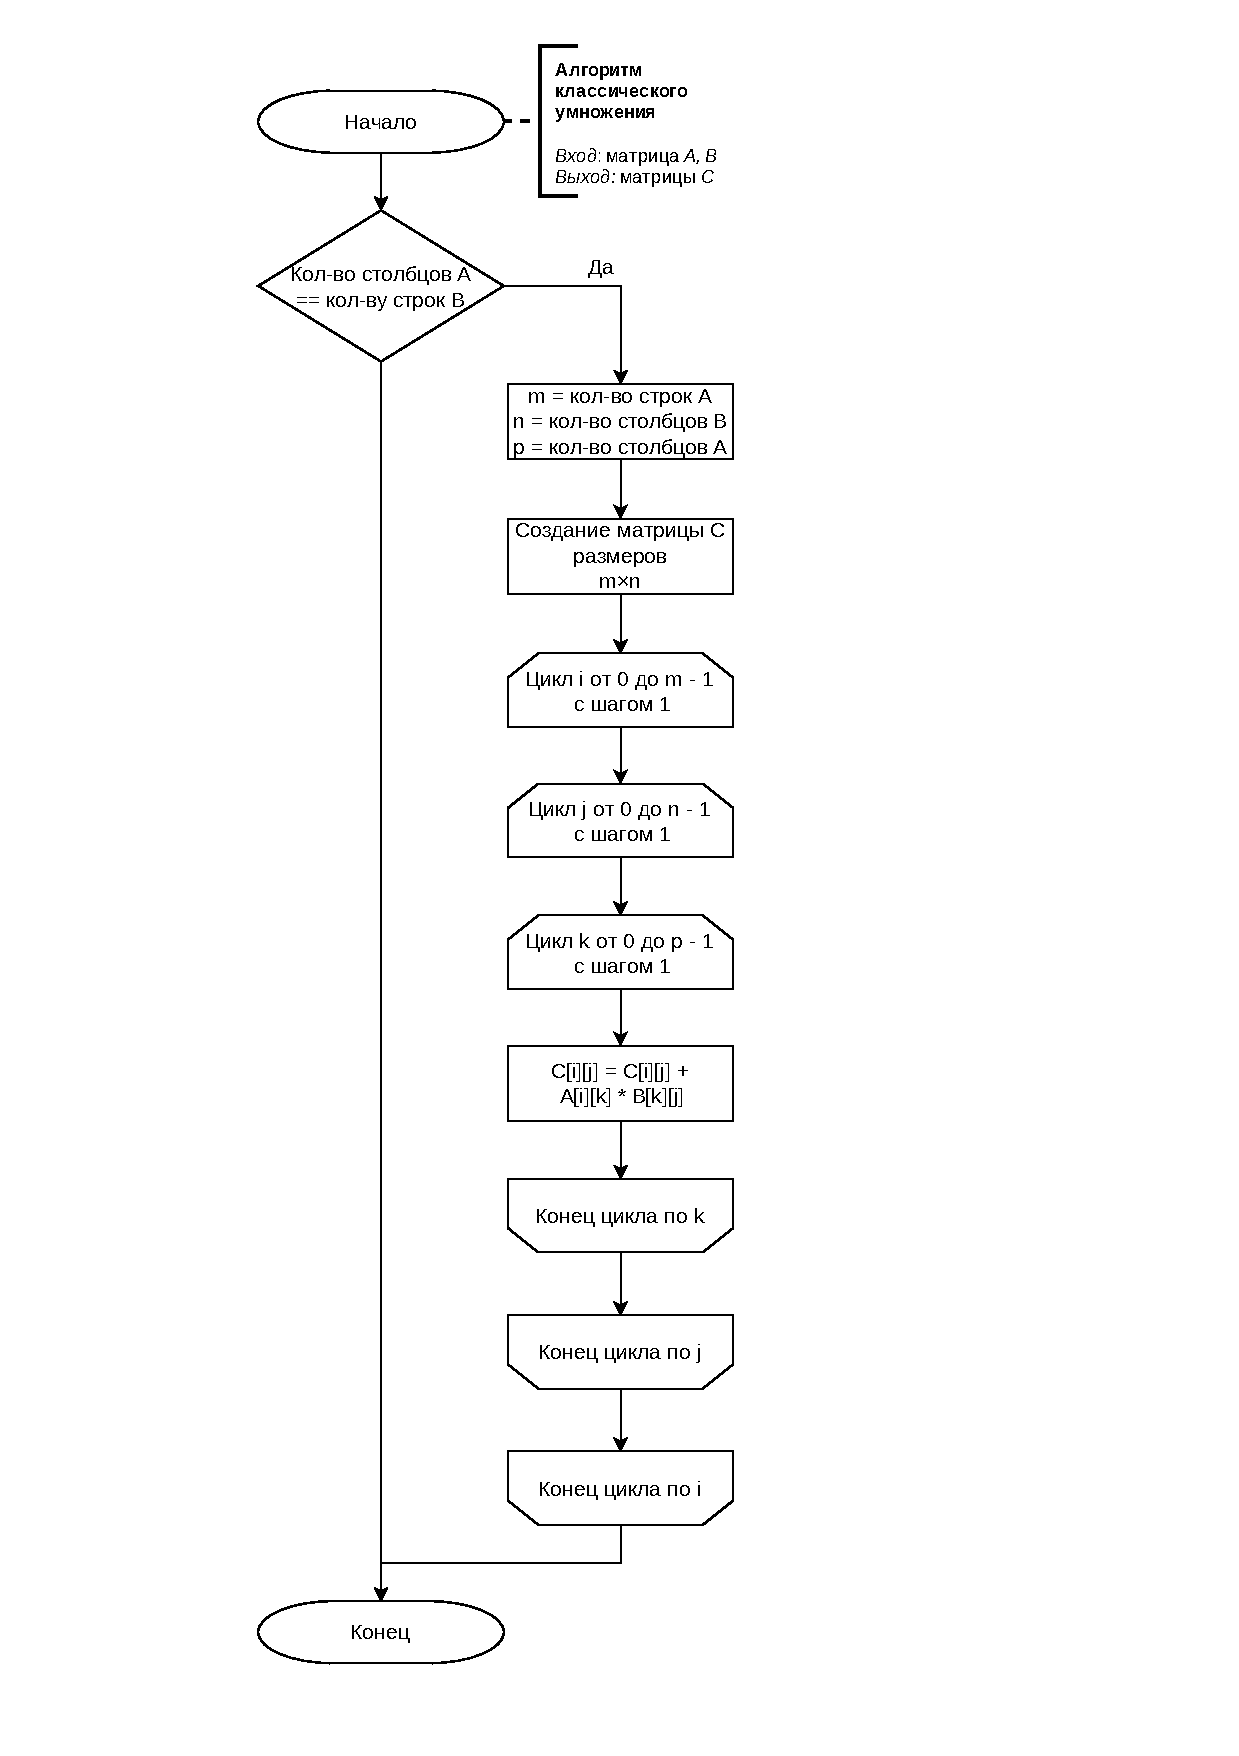
\includegraphics[height=0.7\textheight, page=1]{algo-scheme.pdf}
	\caption{Схема классического алгоритма умножения матриц}
	\label{fig:classic}
\end{figure}

\clearpage

\begin{figure}[h]
	\centering
	\includegraphics[height=0.9\textheight, page=2]{algo-scheme.pdf}
	\caption{Схема алгоритма Винограда (1)}
	\label{fig:vinograd}
\end{figure}

\clearpage

\begin{figure}[h]
	\centering
	\includegraphics[height=0.9\textheight, page=3]{algo-scheme.pdf}
	\caption{Схема алгоритма Винограда (2)}
	\label{fig:vinograd2}
\end{figure}
\clearpage

\begin{figure}[h]
	\centering
	\includegraphics[height=0.9\textheight, page=4]{algo-scheme.pdf}
	\caption{Схема оптимизированного алгоритма Винограда (1)}
	\label{fig:vinograd_opt}
\end{figure}

\begin{figure}[h]
	\centering
	\includegraphics[height=0.9\textheight, page=5]{algo-scheme.pdf}
	\caption{Схема оптимизированного алгоритма Винограда (2)}
	\label{fig:vinograd_opt2}
\end{figure}

\begin{figure}[h]
	\centering
	\includegraphics[height=0.9\textheight, page=6]{algo-scheme.pdf}
	\caption{Схема алгоритма Штрассена}
	\label{fig:strass}
\end{figure}

\clearpage


\section{Описание используемых типов данных}

При реализации алгоритмов будет использована \textit{матрица}~--- двумерный массив \texttt{целочисленного типа}.

\section{Модель вычислений для проведения оценки трудоемкости алгоритмов}

Для последующего вычисления трудоемкости необходимо ввести модель вычислений:

\begin{enumerate}
	\item операции из списка \ref{eq:operations1} имеют трудоемкость \textbf{1};
	\begin{equation}
		\label{eq:operations1}
		\begin{gathered}
			+, -, =, +=, -=, ==, !=, <, >, <=, >=, [], \\ ++, --, \&\&, >>, <<, ||, \&, |
		\end{gathered}
	\end{equation}
	\item операции из списка \ref{eq:operations2} имеют трудоемкость \textbf{2};
	\begin{equation}
		\label{eq:operations2}
		*, /, \%, *=, /=, \%=
	\end{equation}
	\item трудоемкость условного оператора \texttt{if условие then A else B} рассчитывается как \ref{eq:if};
	\begin{equation}
		\label{eq:if}
		f_{if} = f_{\text{условия}} + 
		\begin{cases}
			f_{A}, & \text{в случае выполнеия условия,}\\
			f_{B}, & \text{иначе}.
		\end{cases}
	\end{equation}
	\item трудоемкость цикла рассчитывается как \ref{eq:for}
	\begin{equation}
		\label{eq:for}
		\begin{gathered}
			f_{for} = f_{\text{инициализация}} + f_{\text{сравнения}} + M_{\text{итераций}} \cdot (f_{\text{тело}} +\\
			+ f_{\text{инкремент}} + f_{\text{сравнения}});
		\end{gathered}
	\end{equation}
	\item трудоемкость вызова функции равна 0.
\end{enumerate}

\section{Трудоемкость алгоритмов}
В следующих частях будут приведены рассчеты трудоемкостей алгоритмов для умножения матриц.

Пусть у нас есть 2 матрицы: 
\begin{enumerate}
	\item $A$ размером $M \times P$;
	\item $B$ размером $P \times N$.
\end{enumerate}

\subsection{Стандартный алгоритм}
Трудоемкость стандартного алгоритма умножения матриц состоит из:
\begin{itemize}
	\item внешнего цикла по $i \in [1 \ldots M]$ , трудоемкость которого: $f = 2 + M \cdot (2 + f_{body})$;
	\item цикла по $j \in [1 \ldots N]$ , трудоемкость которого: $f = 2 + N \cdot (2 + f_{body})$;
	\item цикла по $k \in [1 \ldots P]$ , трудоемкость которого: $f = 2 + K \cdot (2 + 12)$;
\end{itemize}
Так как трудоемкость стандартного алгоритма равно трудоемкости внешнего цикла~--- можно вычислить ее, подставив циклы тела:
\begin{equation}
	\begin{gathered}
		f_{standart} = 2 + M \cdot (2 + 2 + N \cdot (2 + 2 + P \cdot (2 + 8 + 1 + 1 + 2))) = \\
		= 2 + 4M + 4MN + 14MNP \approx 14MNP = O(N^3).
	\end{gathered}
\end{equation}

\subsection{Алгоритм Винограда}
При вычислении трудоемкости алгоритма Винограда необходимо учесть следующее:
\begin{itemize}
	\item трудоемкость создания и инициализации массивов \textit{MulH} и \textit{MulV}:
	\begin{equation}
		f_{init} = f_{MulH} + f_{MulV};
	\end{equation}
	\item трудоемкость заполнения массива \textit{MulH}:
	\begin{equation}
		\begin{gathered}
		f_{MulH} = 2 + M \cdot (2 + 4 + \frac{P}{2} \cdot (4 + 6 + 1 + 2 + 3 \cdot 2)) = \\
		= 2 + 6M + \frac{19MP}{2};
		\end{gathered}
	\end{equation}
	\item трудоемкость заполнение массива \textit{MulV}:
	\begin{equation}
		\begin{gathered}
		f_{MulV} = 2 + N \cdot (2 + 4 + \frac{P}{2} \cdot (4 + 6 + 1 + 2 + 3 \cdot 2)) = \\
		= 2 + 6N + \frac{19NP}{2};
		\end{gathered}
	\end{equation}
	\item трудоемкость цикла заполения для четных размеров:
	\begin{equation}
		\begin{gathered}
			f_{cycle} = 2 + M \cdot (4 + N \cdot (13 + \frac{P}{2} \cdot 32)) = 2 + 4M + \\
			+ 13MN + \frac{32MNP}{2}  = 2 + 4M + 13MN + 16MNP;
		\end{gathered}
	\end{equation}
	\item трудоемкость дополнительного цикла, в случае нечетного размера матрицы:
	\begin{equation}
		\begin{gathered}
			f_{check} = 3 + 
			\begin{cases}
				0, & \text{четная} \\
				2 + M \cdot (4 + N \cdot (2 + 14)), & \text{иначе}.
			\end{cases}
		\end{gathered}  
	\end{equation}
\end{itemize}
В итоге, для худшего случая (т. е. когда размер матрицы нечетный) получаем следующую трудоемкость:
\begin{equation}
	f_{worst} = f_{MulH} + f_{MulV} + f_{cycle} + f_{check} \approx 16MNP = O(N^3).
\end{equation}
Для лучшего случая (т. е. когда размер матрицы четный):
\begin{equation}
	f_{best} = f_{MulH} + f_{MulV} + f_{cycle} + f_{check} \approx 16MNP = O(N^3).
\end{equation}

\subsection{Оптимизированный алгоритм Винограда}
Итоговая трудоемкость оптимизированного алгоритма Винограда состоит из:
\begin{itemize}
	\item трудоемкости кеширования значения $\frac{P}{2}$~--- 3;
	\item трудоемкость заполнения массива \textit{MulH}:
	\begin{equation}
		\begin{gathered}
			f_{MulH} = 2 + M \cdot (2 + 2 + \frac{P}{2} \cdot (2 + 5 + 1 + 2 + 3)) = \\
			= 2 + 2M + \frac{13MP}{2};
		\end{gathered}
	\end{equation}
	\item трудоемкость заполнение массива \textit{MulV}:
	\begin{equation}
		\begin{gathered}
			f_{MulV} = 2 + N \cdot (2 + 2 + \frac{P}{2} \cdot (2 + 5 + 1 + 2 + 3)) = \\
			= 2 + 2N + \frac{13NP}{2};
		\end{gathered}
	\end{equation}
	\item трудоемкость цикла заполения для четных размеров:
	\begin{equation}
		\begin{gathered}
			f_{cycle} = 2 + M \cdot (4 + N \cdot (2 + 10 + 2 + \frac{P}{2} \cdot 19)) = \\
			= 2 + 4M + 14MN + \frac{19MNP}{2};
		\end{gathered}
	\end{equation}
	\item трудоемкость дополнительного цикла, в случае нечетного размера матрицы:
	\begin{equation}
		\begin{gathered}
			f_{check} = 3 + 
			\begin{cases}
				0, & \text{четная} \\
				2 + M \cdot (4 + N \cdot (2 + 11)), & \text{иначе}.
			\end{cases}
		\end{gathered}  
	\end{equation}
\end{itemize}
В итоге, для худшего случая (т. е. когда размер матрицы нечетный) получаем следующую трудоемкость:
\begin{equation}
	f_{worst} = f_{MulH} + f_{MulV} + f_{cycle} + f_{check} \approx \frac{19MNP}{2} = O(N^3).
\end{equation}
Для лучшего случая (т. е. когда размер матрицы четный):
\begin{equation}
	f_{best} = f_{MulH} + f_{MulV} + f_{cycle} + f_{check} \approx \frac{19MNP}{2} = O(N^3).
\end{equation}

\subsection{Алгоритм Штрассена}
Если $M(n)$~--- количество умножений, выполняемых алгоритмом для умножения двух матриц размером $n \times n$ (где $n$~--- степень двойки), то получим следующее рекурретное соотношение для $M(n)$:
\begin{equation}
	\begin{gathered}
		M(n) = 7M(\frac{n}{2}).
	\end{gathered}
\end{equation}
При $n > 1, M(1) = 1$. Поскольку $n = 2^{k}$,
\begin{equation}
	\begin{gathered}
		M(2^{k}) = 7M(2^{k - 1}) = 7 \cdot [7M(2^{k - 2})] = 7^{2}M(2^{k - 2}) = \dots = \\ = 7^{i}M(2^{k - i}) = \dots = 7^{k}M(2^{k - k}) = 7^{k}.
	\end{gathered}
\end{equation}
Подставляя $k = \log_{2}n$, получаем:
\begin{equation}
	\begin{gathered}
		M(n) = 7^{\log_{2}n} = n^{\log_{2}7} \approx n^{2.807},
	\end{gathered}
\end{equation}
что меньше, чем $n_{3}$, необходимое для стандартного алгоритма.

Также необходимо рассмотреть количество сложений $A(n)$, выполняемых алгоритмом.
Для умножения двух матриц порядка $n > 1$ алгоритму требуется \textbf{7} умножений и \textbf{18} сложений матриц размером $\frac{n}{2} \times \frac{n}{2}$.
Это сводится к следующему реккурентному уравнению:
\begin{equation}
	\begin{gathered}
		A(n) = 7 \cdot A \cdot \frac{n}{2} + 18 \cdot (\frac{n}{2})^{2}.
	\end{gathered}
\end{equation}
При $ n > 1, A(1) = 0$.

Итоговую трудоемкость можно рассчитать как:
\begin{equation}
	\begin{gathered}
		T(n) = A(n) + M(n).
	\end{gathered}
\end{equation}

\section*{Вывод}
\addcontentsline{toc}{section}{Вывод}

В данном разделе на основе теоретических данных были перечислены требования к ПО, построены схемы реализуемых алгоритмов и представлена модель вычислений на основе данных, полученных на этапе анализа.

\clearpage

\chapter{Технологическая часть}
В данном разделе будут приведены средства реализации, листинг кода и функциональные тесты.

\section{Средства реализации}

В качестве языка программирования, используемого при написании данной лабораторной работы, был выбран C++ \cite{cpp-lang}, так как в нем имеется контейнер \texttt{std::string}, представляющий собой массив символов \texttt{char}, и библиотека \texttt{<ctime>} \cite{ctime}, позволяющая производить замеры процессорного времени.

В качестве среды для написания кода был выбран \textit{Visual Studio Code} за счет того, что она предоставляет функционал для проектирования, разработки и отладки ПО.

\section{Сведения о модулях программы}

Данная программа разбита на следующие модули:

\begin{itemize}
    \item \texttt{main.cpp}~--- точка входа программы, пользовательское меню;
    \item \texttt{general}~--- модуль с определением матрицы;
    \item \texttt{algo}~--- модуль с реализациями алгоритмов умножения матриц;
    \item \texttt{measurement}~--- модуль с реализаций функции подсчета затрачиваемого времени
\end{itemize}

\clearpage

\section{Реализация алгоритмов}

Далее будут представлены реализацим следующих алгоритмов умножения матриц:
\begin{itemize}
    \item \texttt{main.cpp}~--- Классический алгоритм умножения матриц;
    \item \texttt{general}~--- Алгоритм Винограда;
    \item \texttt{algo}~--- Оптимизированный алгоритм Винограда;
    \item \texttt{measurement}~--- Алгоритм Штрассена
\end{itemize}

\begin{lstlisting}[caption=Классический алгоритм умножения матриц]
Matrix mult_classic(const Matrix& matrix1, const Matrix& matrix2)
{
     int rows = matrix1.height, 
        columns = matrix2.width,
        tmp = matrix1.width;

    Matrix res{rows, columns, 0};

    for (int i = 0; i < rows; ++i) {

        for (int j = 0; j < columns; ++j) {
            
            for (int k = 0; k < columns; ++k) {
                res[i][j] = res[i][j] + matrix1[i][k] * matrix2[k][j];
            }
        }
    }

    return res;   
}
\end{lstlisting}
\clearpage

\begin{lstlisting}[caption=Алгоритм Винограда]
Matrix mult_vinograd(const Matrix& matrix1, const Matrix& matrix2)
{
    int rows = matrix1.height;

    Matrix res{rows, rows};

    vector<int> mulH(rows, 0);
    vector<int> mulV(rows, 0);

    for (int i = 0; i < rows; ++i) {

        for (int j = 0; j < rows / 2; ++j) 
            mulH[i] = mulH[i] + matrix1[i][j * 2] * matrix1[i][j * 2 + 1]; 
    }

    for (int i = 0; i < rows; ++i) {

        for (int j = 0; j < rows / 2; ++j) 
            mulV[i] = mulV[i] +  matrix2[j * 2][i] * matrix2[j * 2 + 1][i];
    }

    for (int i = 0; i < rows; ++i) {

        for (int j = 0; j < rows; ++j) {
            
            res[i][j] = -mulH[i] - mulV[j];

            for (int k = 0; k < rows / 2; ++k) 
                res[i][j] = res[i][j] + (matrix1[i][k* 2] + matrix2[k* 2 + 1][j]) * (matrix1[i][k* 2 + 1] + matrix2[k* 2][j]);
        }
    }

    if (rows % 2) {

        for (int i = 0; i < rows; ++i) {

            for (int j = 0; j < rows; ++j) 
                res[i][j] = res[i][j] + matrix1[i][rows - 1] * matrix2[rows - 1][j];
        }
    }

    return res;   
}
\end{lstlisting}
\clearpage

\begin{lstlisting}[caption=Оптимизированный алгоритм Винограда]
int recurs_dam_lev_temp(const char*str1, const char*str2, int length1, int length2)
Matrix mult_vinograd_opt(const Matrix& matrix1, const Matrix& matrix2)
{
    int rows = matrix1.height;

    Matrix res{rows, rows, 0};

    vector<int> mulH(rows, 0);
    vector<int> mulV(rows, 0);

    int stepHalf = rows / 2;

    for (int i = 0; i < rows; ++i) {

        for (int j = 0; j < stepHalf; ++j) 
            mulH[i] = mulH[i] + matrix1[i][(j << 1)] * matrix1[i][(j << 1) + 1]; 
    }

    for (int i = 0; i < rows; ++i) {

        for (int j = 0; j < stepHalf; ++j) 
            mulV[i] = mulV[i] +  matrix2[(j << 1)][i] * matrix2[(j << 1) + 1][i];
    }

    for (int i = 0; i < rows; ++i) {

        for (int j = 0; j < rows; ++j) {
            
            res[i][j] = -mulH[i] - mulV[j];

            for (int k = 0; k < stepHalf; ++k) 
                res[i][j] = res[i][j] + (matrix1[i][(k << 1)] + matrix2[(k << 1) + 1][j]) * (matrix1[i][(k << 1) + 1] + matrix2[(k << 1)][j]);
        }
    }

    if (rows % 2) {

        for (int i = 0; i < rows; ++i) {

            for (int j = 0; j < rows; ++j) 
                res[i][j] = res[i][j] + matrix1[i][rows - 1] * matrix2[rows - 1][j];
        }
    }

    return res;   
}
\end{lstlisting}
\clearpage
\begin{lstlisting}[caption=Алгоритм Штрассена]
Matrix mult_strassen(const Matrix& matrix1, const Matrix& matrix2)
{
    int rows = matrix1.height;
    int n = rows / 2;

    if (rows <= 2)
        return mult_classic(matrix1, matrix2);

    auto a11 = matrix1.slice(0, n, 0, n);
    auto a12 = matrix1.slice(0, n, n, rows);
    auto a21 = matrix1.slice(n, rows, 0, n);
    auto a22 = matrix1.slice(n, rows, n, rows);

    auto b11 = matrix2.slice(0, n, 0, n);
    auto b21 = matrix2.slice(n, rows, 0, n);

    auto b12 = matrix2.slice(0, n, n, rows);
    auto b22 = matrix2.slice(n, rows, n, rows);

    auto p1 = mult_strassen(a11 + a22, b11 + b22);
    auto p2 = mult_strassen(a22, b21 - b11);
    auto p3 = mult_strassen(a11 + a12, b22);
    auto p4 = mult_strassen(a12 - a22, b21 + b22);
    auto p5 = mult_strassen(a11, b12 - b22);
    auto p6 = mult_strassen(a21 + a22, b11);
    auto p7 = mult_strassen(a11 - a21, b11 + b12);

    auto c11 = p1 + p2 - p3 + p4;
    auto c12 = p5 + p3;
    auto c21 = p6 + p2;
    auto c22 = p5 + p1 - p6 - p7;


    return matrix_merge(c11, c12, c21, c22);;
}
\end{lstlisting}
\clearpage
\section{Функциональные тесты}

В данном разделе будут представлены функциональные тесты, проверяющие работу алгоритмов умножения матриц.

В таблице \ref{tbl:func_test_std} приведены тесты для функции, реализующей алгоритм стандартного умножения матриц.

В таблице \ref{tbl:func_test_vin} приведены тесты для функции, реализующей алгоритм умножения матриц методом Винограда.

В таблице \ref{tbl:func_test_strassen} приведены тесты для функции, реализующей алгоритм умножения матриц методом Штрассена.

\begin{table}[h!]
    \caption{Функциональные тесты для стандартного алгоритма умножения матриц}
    \label{tbl:func_test_std}
    \centering
        \begin{tabular}{||c|c|c||} 
        \hline
        Матрица 1& Матрица 2& Ожидаемый результат \\
        \hline\hline
        $\begin{pmatrix}
            1 & 2\\
            3 & 4\\
        \end{pmatrix}$ 
        &  
        $\begin{pmatrix}
            1 \\
            3 \\
        \end{pmatrix}$
        &
        \textit{Неверный размер} \\
        \hline
        $\begin{pmatrix}
            1 & 2\\
        \end{pmatrix}$ 
        &  
        $\begin{pmatrix}
            3 & 4\\
        \end{pmatrix}$
        &
        \textit{Неверный размер} \\
        \hline
        $\begin{pmatrix}
            1
        \end{pmatrix}$ 
        &  
        $\begin{pmatrix}
            1
        \end{pmatrix}$
        &
        $\begin{pmatrix}
            1
        \end{pmatrix}$ \\
        \hline
        $\begin{pmatrix}
            1 & 1 & 1\\
        \end{pmatrix}$ 
        &  
        $\begin{pmatrix}
            1\\
            1\\
            1\\
        \end{pmatrix}$
        &
        $\begin{pmatrix}
            3
        \end{pmatrix}$ \\
        \hline
        $\begin{pmatrix}
            1 & 2 & 3\\
            4 & 5 & 6\\
            7 & 8 & 9\\
        \end{pmatrix}$ 
        &  
        $\begin{pmatrix}
            1 & 0 & 0\\
            0 & 1 & 0\\
            0 & 0 & 1\\
        \end{pmatrix}$
        &
        $\begin{pmatrix}
            1 & 2 & 3\\
            4 & 5 & 6\\
            7 & 8 & 9\\
        \end{pmatrix}$ \\
        \hline
        $\begin{pmatrix}
            1 & 2 & 3\\
            4 & 5 & 6\\
            7 & 8 & 9\\
        \end{pmatrix}$ 
        &  
        $\begin{pmatrix}
            1 & 0\\
            0 & 1\\
            0 & 0\\
        \end{pmatrix}$
        &
        $\begin{pmatrix}
            1 & 2 \\
            4 & 5 \\
            7 & 8 \\
        \end{pmatrix}$ \\
        \hline
        \end{tabular}
\end{table}

\begin{table}[h!]
    \caption{Функциональные тесты для алгоритма умножения матриц методом Винограда}
    \label{tbl:func_test_vin}
    \centering
        \begin{tabular}{||c|c|c||} 
        \hline
        Матрица 1& Матрица 2& Ожидаемый результат \\
        \hline\hline
        $\begin{pmatrix}
            1 & 2\\
            3 & 4\\
        \end{pmatrix}$ 
        &  
        $\begin{pmatrix}
            &
        \end{pmatrix}$
        &
        \textit{Неверный размер} \\
        \hline
        $\begin{pmatrix}
            1 & 2\\
        \end{pmatrix}$ 
        &  
        $\begin{pmatrix}
            3 & 4\\
        \end{pmatrix}$
        &
        \textit{Неверный размер} \\
        \hline
        $\begin{pmatrix}
            1
        \end{pmatrix}$ 
        &  
        $\begin{pmatrix}
            1
        \end{pmatrix}$
        &
        $\begin{pmatrix}
            1
        \end{pmatrix}$ \\
        \hline
        $\begin{pmatrix}
            1 & 1 & 1\\
        \end{pmatrix}$ 
        &  
        $\begin{pmatrix}
            1\\
            1\\
            1\\
        \end{pmatrix}$
        & \textit{Неверный размер} \\
        \hline
        $\begin{pmatrix}
            5 & 6 & 7\\
            4 & 9 & 8\\
            3 & 2 & 1\\
        \end{pmatrix}$ 
        &  
        $\begin{pmatrix}
            1 & 0 & 0\\
            0 & 1 & 0\\
            0 & 0 & 1\\
        \end{pmatrix}$
        &
        $\begin{pmatrix}
            5 & 6 & 7\\
            4 & 9 & 8\\
            3 & 2 & 1\\
        \end{pmatrix}$ \\
        \hline
        $\begin{pmatrix}
            5 & 6 & 7\\
            4 & 9 & 8\\
            3 & 2 & 1\\
        \end{pmatrix}$ 
        &  
        $\begin{pmatrix}
            1 & 0\\
            0 & 1\\
            0 & 0\\
        \end{pmatrix}$
        & \textit{Неверный размер} \\
        \hline
        \end{tabular}
\end{table}

\begin{table}[h!]
    \caption{Функциональные тесты для алгоритма умножения матриц методом Штрассена}
    \label{tbl:func_test_strassen}
    \centering
        \begin{tabular}{||c|c|c||} 
        \hline
        Матрица 1& Матрица 2& Ожидаемый результат \\
        \hline\hline
        $\begin{pmatrix}
            1 & 2\\
            3 & 4\\
        \end{pmatrix}$ 
        &  
        $\begin{pmatrix}
            &
        \end{pmatrix}$
        &
        \textit{Неверный размер} \\
        \hline
        $\begin{pmatrix}
            1 & 2\\
        \end{pmatrix}$ 
        &  
        $\begin{pmatrix}
            3 & 4\\
        \end{pmatrix}$
        &
        \textit{Неверный размер} \\
        \hline
        $\begin{pmatrix}
            1 & 1 & 1\\
        \end{pmatrix}$ 
        &  
        $\begin{pmatrix}
            1\\
            1\\
            1\\
        \end{pmatrix}$
        &
        \textit{Неверный размер} \\
        \hline
        $\begin{pmatrix}
            5 & 6 & 7\\
            4 & 9 & 8\\
            3 & 2 & 1\\
        \end{pmatrix}$ 
        &  
        $\begin{pmatrix}
            1 & 0 & 0\\
            0 & 1 & 0\\
            0 & 0 & 1\\
        \end{pmatrix}$
        &
        \textit{Неверный размер} \\
        \hline
        $\begin{pmatrix}
            1
        \end{pmatrix}$ 
        &  
        $\begin{pmatrix}
            1
        \end{pmatrix}$
        &
        $\begin{pmatrix}
            1
        \end{pmatrix}$ \\
        \hline
        $\begin{pmatrix}
            5 & 7\\
            4 & 8\\
        \end{pmatrix}$ 
        &  
        $\begin{pmatrix}
            1 & 0\\
            0 & 1\\
        \end{pmatrix}$
        &
        $\begin{pmatrix}
            5 & 7\\
            4 & 8\\
        \end{pmatrix}$ \\
        \hline
        $\begin{pmatrix}
            1 & 2 & 3 & 4\\
            5 & 6 & 7 & 8\\
            9 & 10 & 11 & 12\\
            13 & 14 & 14 & 16
        \end{pmatrix}$ 
        &  
        $\begin{pmatrix}
            1 & 0 & 0 & 0\\
            0 & 1 & 0 & 0\\
            0 & 0 & 1 & 0\\
            0 & 0 & 0 & 1
        \end{pmatrix}$
        &
        $\begin{pmatrix}
            1 & 2 & 3 & 4\\
            5 & 6 & 7 & 8\\
            9 & 10 & 11 & 12\\
            13 & 14 & 14 & 16
        \end{pmatrix}$ \\
        \hline
        \end{tabular}
\end{table}

\clearpage

\addcontentsline{toc}{section}{Вывод}
\section*{Вывод}

Были реализованы классический алгоритм умножения матриц, алгоритм Винограда и его оптимизированная версия, алгоритм Штрассена.
Проведено тестирование реализованных алгортимов.

\clearpage

\chapter{Исследовательская часть}

\section{Технические характеристики}
Технические характеристики устройства, на котором выполнялись
замеры по времени:

\begin{itemize}
    \item Процессор: Intel Core i7 9750H 2.6 ГГц;
    \item Оперативная память: 16 ГБ;
    \item Операционная система: Kubuntu 22.04.3 LTS x86\_64 Kernel: 6.2.0-36-generic
\end{itemize}

Во время проведения измерений времени ноутбук был подключен к сети электропитания и был нагружен только системными приложениями.

\section{Демонстрация работы программы}

На рисунке \ref{fig:img_prog} показан пример работы с программой.


\begin{figure}[ht!]
	\centering
	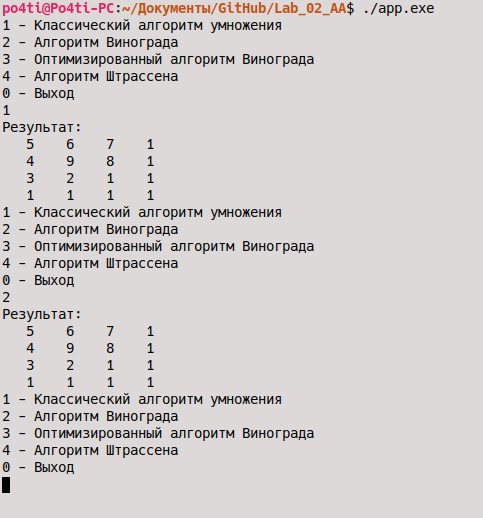
\includegraphics[width=170mm]{img/img_prog.png}
	\caption{Демонстрация работы программы.\label{overflow}}
	\label{fig:img_prog}
	\end{figure}


\clearpage

\section{Временные характеристики}


Исследование временных характеристик реализованных алгоритмов производилось на квадратных матрицах размерами:

\begin{itemize}
    \item 1 -- 128 c шагом 1 без алгоритма штрассена;
    \item 1 -- 128 с увеличением шага в 2 раза для всех алгоритмов
\end{itemize}

% \begin{figure}[H]
%     \includesvg[width=1.0\textwidth]{img/plotting_data1.svg}
%     \caption{Результат измерений времени работы (в мс) нерекурсивных реализаций алгоритмов поиска расстояний Левенштейна и Дамерау~---~Левенштейна}
%     \label{fig:plotting_data1}
% \end{figure}

% \begin{figure}[H]
%     \includesvg[width=1.0\textwidth]{img/plotting_data2.svg}
%     \caption{Результат измерений времени работы рекурсивных реализаций алгоритма поиска расстояния Дамерау~---~Левенштейна}
%     \label{fig:plotting_data2}
% \end{figure}

На рисунке \ref{fig:nonstrassen} показаны зависимости времени выполнения всех алгоритмов, кроме алгоритма Штрассена от размера матриц.

На рисунке \ref{fig:strassen} показаны зависимости времени выполнения всех алгоритмов от размера матриц.


\begin{figure}[H]
    \centering
    \includesvg[width=1.0\textwidth]{img/plotting_data1.svg}
    \caption{Результат измерений времени работы реализуемых алгоритмов на матрицах с шагом размера 1}
    \label{fig:nonstrassen}
\end{figure}


\begin{figure}[H]
    \centering
    \includesvg[width=1.0\textwidth]{img/plotting_data2.svg}
    \caption{Результат измерений времени работы реализуемых алгоритмов на матрицах, размеры которых~--- степень 2}
    \label{fig:strassen}
\end{figure}

\section{Характеристики по памяти}
Введем следующие обозначения:
\begin{itemize}
	\item $size()$~--- функция вычисляющая размер в байтах;
	\item $int$~--- целочисленный тип
\end{itemize}

Приведем теоретический расчет затрат по памяти для умножения двух матриц $A$ и $B$ размером $n \times n$, элементы которых типа $int$.

\subsection*{Стандартный алгоритм}
Затраты по памяти для реализации стандартного алгоритма приведены в формуле \ref{eq:mem_std}:
\begin{equation}
	\label{eq:mem_std}
	\begin{gathered}
		M_{std} = 3 \cdot size(int) + 3 \cdot size(int) + n \cdot n \cdot size(int) = \\ = (n^{2} + 6) \cdot size(int),
	\end{gathered}
\end{equation}
где, $3 \cdot size(int)$~--- переменные, хранящие размеры матриц;
\newline $3 \cdot size(int)$~--- переменные, используемые в циклах;
\newline $n \cdot n \cdot size(int)$~--- результирующая матрица.

\subsection*{Алгоритм Винограда}
Затраты по памяти для реализации алгоритма умножения методом Винограда приведены в формуле \ref{eq:mem_vin}:
\begin{equation}
	\label{eq:mem_vin}
	\begin{gathered}
		M_{vin} = M_{mulH} + M_{mulV} + M_{mul},
	\end{gathered}
\end{equation}
где $M_{mulH}, M_{mulV}$~--- память, используемая для хранения дополнительных массивов;
\newline $M_{mul}$~--- память, используемая при самом умножении матриц;

Соответствующие затраты представлены в формулах \ref{eq:mem_vin_1}--\ref{eq:mem_vin_2}
\begin{equation}
	\label{eq:mem_vin_1}
	\begin{gathered}
		M_{mulH} = M_{mulV} = n \cdot size(int) + 2 * size(int);
	\end{gathered}
\end{equation}
\begin{equation}
	\label{eq:mem_vin_2}
	\begin{gathered}
		M_{mul} = n \cdot n \cdot size(int) + 3 \cdot size(n) +
			\begin{cases}
				0, & \text{четная} \\
				2 \cdot size(int), & \text{иначе}.
			\end{cases}
	\end{gathered}
\end{equation}

Итоговые затраты по памяти для реализации алгоритма Винограда:
\begin{equation}
	\label{eq:mem_vin_res}
	\begin{gathered}
		M_{mul} = (n^{2} + 2 \cdot n + 7) \cdot size(int) +
			\begin{cases}
				0, & \text{четная} \\
				2 \cdot size(int), & \text{иначе}.
			\end{cases}
	\end{gathered}
\end{equation}

\subsection*{Оптимизированнный алгоритм Винограда}
Затраты по памяти для оптимизированной реализации алгоритма умножения методом Винограда идентичны формуле \ref{eq:mem_vin}.
$M_{mulH}$ и $M_{mulV}$ для данной релизации также совпадают.

Отличия появляются в самом умножении матриц, поскольку в целях оптимизации необходимо было некоторые значения хранить в отдельных переменных.
\begin{equation}
	\label{eq:mem_vinopt}
	\begin{gathered}
		M_{mul} = n \cdot n \cdot size(int) + 4 \cdot size(n) + \\ + n \cdot n \cdot \frac{n}{2} * size(int) + n \cdot n * size(int)
			\begin{cases}
				0, & \text{четная} \\
				2 \cdot size(int), & \text{иначе}.
			\end{cases}
	\end{gathered}
\end{equation}

Итоговые затраты по памяти для оптимизированной реализации алгоритма Винограда:
\begin{equation}
	\label{eq:mem_vinopt_res}
	\begin{gathered}
		M_{mul} = (\frac{n^{3}}{2} + 2 \cdot n^{2} + 6 \cdot n + 4) \cdot size(int) +
		\begin{cases}
			0, & \text{четная} \\
			2 \cdot size(int), & \text{иначе}.
		\end{cases}
	\end{gathered}
\end{equation}

\subsection*{Алгоритм Штрассена}
Рассчитаем затраты по памяти для каждого рекурсивного вызова.
\begin{equation}
	\label{eq:mem_stras}
	\begin{gathered}
		M_{mul} = (4 \cdot \frac{n}{2} \cdot \frac{n}{2} + 4 \cdot \frac{n}{2} \cdot \frac{n}{2} + \\ + 21 \cdot \frac{n}{2} \cdot \frac{n}{2} + n \cdot n) \cdot size(int),
	\end{gathered}
\end{equation}
где $4 \cdot \frac{n}{2} \cdot \frac{n}{2}$~--- 4 матрицы, на которые мы разбиваем нашу исходную матрицу;
\newline $13 \cdot \frac{n}{2} \cdot \frac{n}{2}$~--- временные матрицы, получаемые в ходе вычислений;
\newline $n \cdot n$~--- результирующая матрица.

Итоговые затраты по памяти для реализации алгоритма Штрассена:
\begin{equation}
	\label{eq:mem_stras_res}
	\begin{gathered}
		M_{mul} = \frac{33}{4} \cdot n^{2} \cdot size(int).
	\end{gathered}
\end{equation}
\addcontentsline{toc}{section}{Вывод}
\section*{Вывод}
Исходя из данных, полученных с помощью графиков \ref{fig:nonstrassen} --\ref{fig:strassen} , можно сделать вывод, что лучше всего работает отмизированный алгоритм Винограда.
Стандартный же алгоритм умножения матриц работает медленнее по сравнению с двумя реалазиями алгоритма Винограда.
Модификации, используемые в оптимизированной реализации алгоритма также повлияли на его скорость работы. 
Также алгоритм Винограда при четном размере матрицы работает быстрее~--- это обусловлено проведением дополнительных вычислений для крайних строк и cтолбцов при нечетном размере. 
Таким образом, алгоритм Винограда стоит использовать при работе именно с матрицами, размер которых~--- четный.

Также на рис. \ref{fig:strassen} видно, что реализация алгоритма Штрассена выполняется намного дольше реализации алгоритма Винограда, так как он требует дополнительных операций сложения и вычитаний матриц.

Из теоретических расчетов для потребляемой памяти, можно сделать вывод о том, что стандартное умножение требует наименьшее количество памяти. 
Наибольшие же затраты требует реализация алгоритма Штрассена, так как при каждом рекурсивном вызове необходимо разбивать исходные матрицы на 4 подматрицы, а также производить дополнительные опериции сложения и умножения.
Оптимизированная реализация алгоритма также требует больше памяти, по сравнению с неоптимизированной, так как используются дополнительные переменные для хранения некоторых предварительных вычислений.

\chapter*{Заключение}
\addcontentsline{toc}{chapter}{Заключение}

В ходе исследования было определено, что оптимизированный алгоритм Винограда продемонстрировал лучшую производительность. 
Классический метод умножения матриц работает медленнее по сравнению с остальными рассмотренными алгоритмами. 
Кроме того, реализация алгоритма Штрассена требует больше времени на выполнение из-за дополнительных операций сложения и вычитания матриц.
Среди всех рассмотренных алгоритмов, наименьшую сложность имеет алгоритм штрассена - $O(N^{2.807})$, в то время как остальные - $O(N^3)$.

С учетом расчетов потребляемой памяти можно сделать вывод о том, что стандартное умножение требует наименьшее количество памяти, а алгоритм Штрассена требует наибольших затрат памяти из-за создания дополнительных матриц при каждом рекурсивном вызове, а также дополнительных операций сложения и умножения. 
Оптимизированная реализация алгоритма Винограда также требует больше памяти по сравнению с неоптимизированной из-за использования дополнительных переменных для хранения некоторых предварительных вычислений. 

Цель данной лабораторной работы была достигнута -- был проведен анализ алгоритмов умножения матриц.

В результате выполнения лабораторной работы для достижения этой цели были выполнены следующие задачи:
\begin{enumerate}
    \item Изучены следующие алгоритмы: %поиска расстояния Левенштейна и Дамерау~---~Левенштейна.
    \begin{itemize}    
        \item классический алгоритм умножения;
        \item алгоритм Винограда;
        \item алгоритм Штрассена;        
        \item оптимизированный алогритм Винограда
    \end{itemize}
    \item Реализованы алгоритмы умножения матриц;%поиска редакционных расстояний.
    \item Выполнены замеры затрат реализаций алгоритмов по памяти;
    \item Выполнены замеры затрат реализаций алгоритмов по процессорному времени;
    \item Проведен сравнительных анализ алгоритмов
\end{enumerate}
